\documentclass{article}
\usepackage{amsmath, graphicx} % For advanced math environments
\usepackage{xcolor}
\usepackage{titlesec}
\usepackage{setspace}
\usepackage[a4paper, left=3cm, right=3cm, top=2cm, bottom=2cm]{geometry}
\title{9.4 Models for Population Growth}
\author{}
\date{}
\setstretch{1.2} % 문서 전체 줄 간격을 1.5배로 설정
\graphicspath{{graph/}}

% \section의 형식을 지정
% 형식: \titleformat{\section}{<모양>}{<번호>}{<번호와 제목 간격>}{<색상 등 제목 스타일>}
\titleformat{name=\section, numberless}
  {\normalfont\Large\bfseries\color{blue}} % 글꼴, 크기, 굵기, 색상
  {} % 섹션 번호
  {1em}        % 번호와 제목 사이 간격
  {}           % 제목 텍스트 (여기서는 비워둠)
\geometry{a4paper, margin=1in}

\begin{document}
\maketitle

This section expands on the population growth models introduced in Section 9.1, using techniques from Section 9.3 to derive explicit formulas for population dynamics.

\section*{The Law of Natural Growth}

One basic model assumes that population growth rate is proportional to the population size:
\[\frac{dP}{dt} = kP\]
where $k$ is a constant.
This is known as the law of natural growth. If $k>0$, the population increases; if $k<0$, it decreases.\\
\\This is a separable differential equation. Solving it yields:
\[P(t) = A e^{kt}\]
where $A$ is an arbitrary constant.\\
Since $P(0)=A$, $A$ represents the initial population $P_0$.
Thus, the solution to the initial-value problem $\frac{dP}{dt} = kP$, $P(0)=P_0$ is:
\[P(t) = P_0 e^{kt}\]
This model implies a constant relative growth rate ($\frac{dP/dt}{P} = k$), leading to exponential growth.

\section*{The Logistic Model}

A more realistic model accounts for limited resources and a carrying capacity $M$, the maximum population an environment can sustain. 
The relative growth rate decreases as population $P$ increases. 
This leads to the logistic differential equation:
\[\frac{dP}{dt} = kP\left(1 - \frac{P}{M}\right)\]
If $P$ is small compared to $M$, $\frac{dP}{dt} \approx kP$ (exponential growth).
\\If $P > M$, $1 - P/M$ is negative, so $\frac{dP}{dt} < 0$ and the population decreases.
\\Equilibrium solutions are $P(t) = 0$ and $P(t) = M$, where $\frac{dP}{dt} = 0$.

\subsubsection*{Example 1: Direction Field for Logistic Equation}
Draw a direction field for the logistic equation with $k = 0.08$ and carrying capacity $M = 1000$. 
What can be deduced about the solutions?

\paragraph{Solution:}
The equation is $\frac{dP}{dt} = 0.08P\left(1 - \frac{P}{1000}\right)$.
The direction field shows positive slopes for $0 < P < 1000$ and negative slopes for $P > 1000$.
Slopes are small near $P=0$ and $P=1000$. Solutions move away from $P=0$ and toward $P=1000$.
\\Solutions starting below $P=1000$ are increasing, and those starting above $P=1000$ are decreasing. 
Inflection points occur when $P=M/2=500$, where growth is fastest.
\\we use the direction field to sketch solution curves with initial populations $P(0)=100$, $P(0)=400$, $P(0)=13000$.
\\The slope are greatest when $P \approx 500$ and the solution curves that start below $P=1000$ have inflection points when $P \approx 500$. 
we can prove that all solution curves that start below $P=500$ have an inflection point when $P$ is exactly 500.
\begin{figure}[htbp] % [h!] 옵션은 여기에(here!) 그림을 위치시키라는 의미
  \centering % 이미지를 가운데로 정렬
  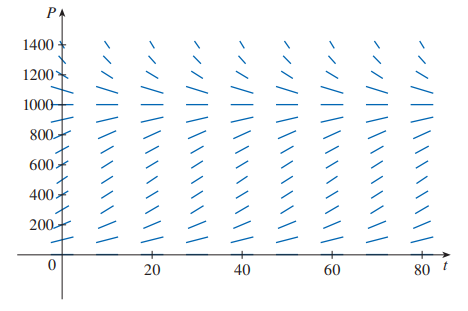
\includegraphics[width=0.4\textwidth]{graph1.png} % 너비는 텍스트 너비의 70%    
  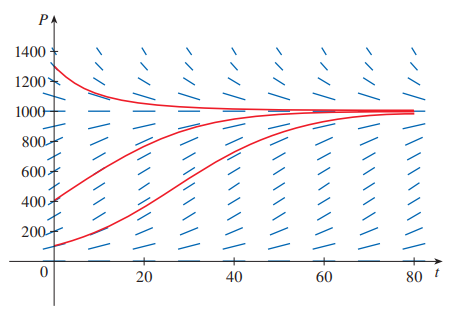
\includegraphics[width=0.4\textwidth]{graph2.png}
\end{figure}
The logistic equation is separable. 
Solving it explicitly using partial fractions yields the solution:
Separating variables:
\[\frac{M}{P(M - P)} dP = k \, dt\]
Now, we use partial fractions for the left side:
\[\frac{M}{P(M - P)} = \frac{1}{P} + \frac{1}{M - P}\]
Integrating both sides:
\[\int \left(\frac{1}{P} + \frac{1}{M - P}\right) dP = \int k \, dt\]
\[\ln|P| - \ln|M - P| = kt + C\]
\[\ln\left|\frac{M - P}{P}\right| = -kt - C\]
Exponentiating both sides:
\[\frac{M - P}{P} = A e^{-kt} \quad (\text{where } A = \pm e^{-C})\]
To solve for $P$:
\[P(t) = \frac{M}{1 + A e^{-kt}}\]
Let $A_0 = A$. Then $P(t) = \frac{M}{1 + A_0 e^{-kt}}$
To find $A_0$ in terms of initial population $P_0$:
At $t=0$, $P(0) = P_0$:
\[P_0 = \frac{M}{1 + A_0} \quad \Rightarrow \quad A_0 = \frac{M - P_0}{P_0}\]
Thus, the solution is:
\[P(t) = \frac{M}{1 + \left(\frac{M - P_0}{P_0}\right) e^{-kt}}\]
This is often written as:
\[P(t) = \frac{M}{1 + A e^{-kt}}, \quad \text{where } A = \frac{M - P_0}{P_0}\]
As expected, $\lim_{t \to \infty} P(t) = M$.

\subsubsection*{Example 2: Applying the Logistic Model}
Write the solution of the initial-value problem $\frac{dP}{dt} = 0.08P\left(1 - \frac{P}{1000}\right)$, $P(0) = 100$. Use it to find $P(40)$ and $P(80)$. At what time does the population reach 900?

\paragraph{Solution:}
Given $k = 0.08$, $M = 1000$, $P_0 = 100$.
\[A = \frac{1000 - 100}{100} = 9\]
So,
\[P(t) = \frac{1000}{1 + 9e^{-0.08t}}\]
\[P(40) = \frac{1000}{1 + 9e^{-3.2}} \approx 731.6\]
\[P(80) = \frac{1000}{1 + 9e^{-6.4}} \approx 985.3\]
To find when $P(t) = 900$:
\begin{align*}
900 &= \frac{1000}{1 + 9e^{-0.08t}} \\
1 + 9e^{-0.08t} &= \frac{1000}{900} = \frac{10}{9} \\
9e^{-0.08t} &= \frac{10}{9} - 1 = \frac{1}{9} \\
e^{-0.08t} &= \frac{1}{81} \\
-0.08t &= \ln\left(\frac{1}{81}\right) = -\ln(81) \\
t &= \frac{\ln(81)}{0.08} \approx 54.9
\end{align*}
The population reaches 900 at approximately $t \approx 55$.

\section*{Comparison of the Natural Growth and Logistic Models}

\subsubsection*{Example 3: Gause's Paramecium Data}
Find the exponential and logistic models for G. F. Gause's Paramecium data (initial relative growth rate $k = 0.7944$, carrying capacity $M = 64$, initial population $P_0 = 2$). Compare predicted values with observed values.

\paragraph{Solution:}
Exponential Model: $P(t) = 2e^{0.7944t}$ \\
Logistic Model:
\[A = \frac{64 - 2}{2} = 31\]
\[P(t) = \frac{64}{1 + 31e^{-0.7944t}}\]
\begin{figure}[htbp] % [h!] 옵션은 여기에(here!) 그림을 위치시키라는 의미
  \centering % 이미지를 가운데로 정렬
  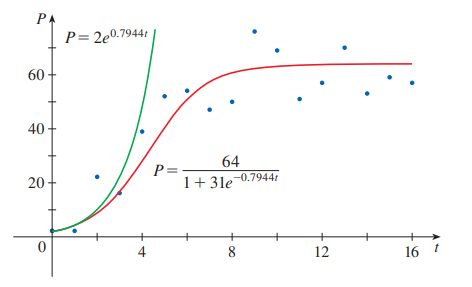
\includegraphics[width=0.4\textwidth]{graph3.png} % 너비는 텍스트 너비의 70%    
\end{figure}
\begin{figure}[htbp] % [h!] 옵션은 여기에(here!) 그림을 위치시키라는 의미
  \centering % 이미지를 가운데로 정렬
  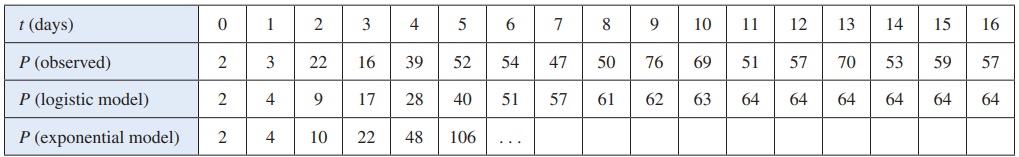
\includegraphics[width=1
  \textwidth]{graph4.png} % 너비는 텍스트 너비의 70%    
\end{figure}
\\It shows that the exponential model is accurate for the first few days but becomes highly inaccurate later, while the logistic model fits the observations reasonably well, especially as the population approaches the carrying capacity.

\section*{Other Models for Population Growth}
Beyond the natural growth and logistic models, other variations exist:
\begin{description}
    \item[Harvesting Model:] $\frac{dP}{dt} = kP\left(1 - \frac{P}{M}\right) - c$ (where $c$ is a constant harvesting rate).
    \item[Minimum Population Level:] $\frac{dP}{dt} = kP\left(1 - \frac{P}{M}\right)\left(1 - \frac{P}{m}\right)$ (where $m$ is a minimum population level below which the species goes extinct).
    \item[Gompertz Function:] $\frac{dP}{dt} = c \ln\left(\frac{P}{M}\right) P$
    \item[Seasonal-Growth Models:] Incorporate periodic functions of time to account for seasonal variations in growth rate.
\end{description}
These models are explored in various exercises and provide more nuanced descriptions of population dynamics.

\end{document}